%\documentclass[11pt,a4paper]{article}
%\usepackage{fullpage}
%\usepackage{beamerarticle}
%\documentclass[handout,xcolor=pdftex,dvipsnames,table]{beamer}
\documentclass[hyperref={unicode=true}]{beamer}

%\usepackage{pgfpages} 
%\pgfpagesuselayout{resize}[a4paper,border shrink=5mm,landscape] 

\usepackage[utf8]{inputenc}
\usepackage[russian]{babel}
\usepackage{../clrscode3e} 
%\usepackage[all]{xy}
\usepackage{colortbl}
%\usepackage{xcolor}
\usepackage{pstricks, pst-tree, pst-node}
\usepackage{epsfig}
\usepackage{multicol}
\usepackage{array}
%\usepackage{listings}

\definecolor{orange}{cmyk}{0,0.52,1,0}

%\usepackage{beamerthemesplit}

\AtBeginSection[]
{
  \begin{frame}<beamer>{Раздел}
    \tableofcontents[currentsection]
  \end{frame}
}


\AtBeginSubsection[]
{
  \begin{frame}<beamer>{Раздел}
    \tableofcontents[currentsection,currentsubsection]
  \end{frame}
}


\newtheorem{rtheorem}{Теорема} 
\newtheorem{rconsequence}{Следствие} 
%default}
%themesplit}

\title{Быстрое преобразование Фурье}
\subtitle{Дискретный анализ 2012/13}
\author{Андрей Калинин, Татьяна Романова}
\date{2 марта 2013\,г.}
\usetheme{default}
%\usefonttheme{serif}
\usefonttheme[onlymath]{serif}
%\usefonttheme{professionalfonts}
%\usetheme{default} 


\begin{document}

\frame{\titlepage}

%\section[Содержание]{}
%\frame{\tableofcontents}
\section{Полиномы и быстрое преобразование Фурье}

%\section{Литература}
\frame
{
  \frametitle{Литература}


  \begin{itemize}
  \item  Кормен Т., Лейзерсон Ч., Ривест Р., Штайн К.. Алгоритмы:
    построение и анализ, 2-е издание, М.:Вильямс, 2005, стр. 926-953, 
    глава 30, <<Полиномы и быстрое преобразование Фурье>>
%  \item Дональд Кнут, <<Искусство программирования>>, том 2,
%    <<Получисленные алгоритмы>>, 3-е издание. Глава 4{.}3,
%    <<Арифметика многкратной точности>>, стр. 304--335. 
  \end{itemize}
}


%\section{Полиномы и быстрое преобразование Фурье}
\frame{
  \frametitle{Полином}
\[
A(x)=\sum^{n-1}_{j=0}a_jx^j
\]
\begin{itemize}
  \item $a_0,a_1, \ldots a_{n-1}$ --- коэффициенты. 
  \item Степень $k$, если $a_k \neq 0$ и $\forall j>k \Rightarrow a_j=0$.
  \item Граница степени $n > k$.
\end{itemize}
}

\frame{
  \frametitle{Операции над полиномами}
\[
\begin{split}
A(x)&=\sum_{j=0}^{n-1}a_jx^j, \qquad B(x)=\sum_{j=0}^{n-1}b_jx^j \\
C(x)&=A(x)+B(x)=\sum_{j=0}^{n-1}(a_j+b_j)x^j=\sum_{j=0}^{n-1}c_jx^j \\
C(x)& =A(x)\times
B(x)=\sum_{j=0}^{2n-2}\left(\sum_{k=0}^ja_kb_{j-k}\right)x^j=\sum_{j=0}^{2n-2}c_jx^j
\end{split}
\]
Вектор коэффициентов умножения, $c=(c_0,c_1,\ldots,c_{2n-2})$
называется свёрткой векторов $a$ и $b$: $a\otimes b$.
}


\subsection{Представление полиномов}

\frame{
  \frametitle{Представление, основанное на коэффицентах}
  \begin{itemize}
  \item Полином $A(x)$ степени не выше $n$ представляется вектором
    коэффициентов:
\[
a = (a_0, a_1, \ldots, a_{n-1})
\]
\item Операция вычисления полинома $A(x)$ в $x_0$ по схеме Горнера
  требует $\Theta(n)$ времени:
\[
A(x_0)=((\cdots((a_{n-1})x_0+a_{n-2})x_0+\cdots + a_2)x_0+a_1)x_0+a_0
\]
\item Сложение полиномов $a$ и $b=(b_0,b_1,\ldots,b_{n-1})$ занимает
  время $\Theta(n)$: 
  \[
  c=(a_0+b_0,a_1+b_1,\ldots,a_{n-1}+b_{n-1})
  \]
\item Умножение наивным способом занимает $\Theta(n^2)$ времени. 
  \end{itemize}
}

\frame{
  \frametitle{Представление, основанное на значениях в точках}
  Множество из $n$ пар точка-значение:
\[
\{(x_0, y_0), (x_1,y_1),\ldots, (x_{n-1},y_{n-1})\}, \qquad x_i\neq x_j
\quad (i\neq j),
\]
$y_k=A(x_k), k=0,1,\ldots,n-1$.
\begin{itemize}
  \item Возможно бесконечное число различных <<точечных>>
    представлений полинома, т.к. можно использовать в качестве базиса
    любые $n$ различных точек. 
  \item Получение по вектору коэффициентов точечного представления ---
    аппроксимация. По схеме Горнера выполняется за $\Theta(n^2)$
    времени. Можно ускорить до $\Theta(n\lg n)$
  \item Определение коэффициентов полинома по точечному представлению
    --- интерполяция.
\end{itemize}
}

\frame{
  \frametitle{Единственность интерполяционного полинома}
  \begin{rtheorem}
    Для любого множества, состоящего из $n$ пар точка-значение
    $\{(x_0,y_0), (x_1,y_1),\ldots,(x_{n-1},y_{n-1})\}$, таких что все
    значения $x_k$ различны, существует единственный полином $A(x)$ с
    границей степени $n$, такой что $y_k=A(x_k)$ для $k=0,1,\ldots,n-1$.
  \end{rtheorem}
}

\frame[plain]{
  \begin{proof}
\[
    \left( 
\begin{array}{ccccc}
1 & x_0 & x_0^2 & \ldots & x_0^{n-1} \\
1 & x_1 & x_1^2 & \ldots & x_1^{n-1} \\
\vdots & \vdots & \vdots & \ddots & \vdots \\
1 & x_{n-1} & x^2_{n-1} & \ldots & x_{n-1}^{n-1}
\end{array}
\right)
\left(
\begin{array}{c}
a_0 \\
a_1 \\
\vdots \\
a_{n-1}
\end{array}
\right) = 
\left(
\begin{array}{c}
y_0 \\
y_1 \\
\vdots \\
y_{n-1}
\end{array}
\right)
\]
Матрица в левой части --- матрица Вандермонда, $V(x_0, x_1, \ldots,
x_{n-1})$:
\[
\det V(x_0,x_1,\ldots, x_{n-1}) = \prod_{0\leq j<k\leq n-1}(x_k-x_j)
\]
следовательно, она обратима если все $x_k$ различны, т.е. можно
однозначно решить уравнение:
\[
a = V(x_0, x_1, \ldots, x_{n-1})^{-1}y
\]
  \end{proof}
}

\frame{
  \frametitle{Формула Лагранжа}
  \[
  A(x)=\sum_{k=0}^{n-1}y_k\frac{\prod_{j\neq k}(x-x_j)}{\prod_{j\neq k}(x_k-x_j)}
\]
Тем самым, можно вычислить коэффциенты полинома $A$ за время $\Theta(n^2)$
}

\frame{
  \frametitle{Операции над полиномами в точечном представлении}
  \[
\begin{array}{c}
  A = \{ (x_0, y_0), (x_1, y_1), \ldots, (x_{n-1},y_{n-1})\},\\
  B = \{ (x_0, y'_0), (x_1, y'_1), \ldots, (x_{n-1},y'_{n-1})\},\\
\end{array}
\]
  \begin{itemize}
    \item Сложение:
\[
\{ (x_0, y_0+y'_0), (x_1, y_1+y'_1), \ldots, (x_{n-1},y_{n-1}+y'_{n-1})\}
\]
\item Умножение требует доопределения значений полиномов до $2n$
  точек, тогда:
\[
\{ (x_0, y_0y'_0), (x_1, y_1y'_1), \ldots, (x_{2n-1},y_{2n-1}y'_{2n-1})\}
\]
    
  \end{itemize}
}

\frame{
  \frametitle{Быстрое умножение полиномов в коэффициентах}
  \begin{itemize}
  \item Наивное перемножение, $\Theta(n^2)$.
  \item Перевод в точечную форму и перемножение там:
    \begin{enumerate}
    \item Удвоение границы степени.
    \item Аппроксимация, $\Theta(n\lg n)$, дискретное преобразование
      Фурье (ДПФ, DFT), в качестве точек выбираются корни мнимой
      единицы степени $2n$: $\omega_{2n}$. Используется метод быстрого
      преобразования Фурье (БПФ). 
    \item Перемножение, $\Theta(n)$.
    \item Интерполяция, $\Theta(n\lg n)$, вычисление обратного ДПФ. 
    \end{enumerate}
  \end{itemize}
  \begin{rtheorem}
    Произведение двух полиномов степенью не выше $n$, представленных в
    коэффициентной форме, можно вычислить за время $\Theta(n\lg n)$.
\end{rtheorem}
}

\subsection{Дискретное преобразование Фурье}

\frame{
  \frametitle{Комплексные корни из единицы}
  Комплексный корень $n$-й степени из единицы число $\omega_n$, такое,
  что 
\[
\omega_n^n=1
\]
Существует ровно $n$ комлексных корней $n$-й степени из 1:
\[
\omega_{n,k}=e^{2\pi i k/n}
\]
При этом значение 
\[
\omega_n=e^{2\pi i/n}
\]
называется главным значением корня $n$-й степени из единицы; тогда все
корни:
\[
\omega^0_n, \omega^1_n, \ldots, \omega^{n-1}_n
\]
образуют группу относительно операции умножения:
\[
\omega^j_n\omega^k_n=\omega^{(j+k)\mod n}_n, \qquad
\omega^{-1}_n=\omega^{n-1}_n
\]
}

\begin{frame}
  \frametitle{Расположение мнимых корней из единицы на комплексной
    плоскости}
  \begin{columns}[T]
    \begin{column}{.6\textwidth}
      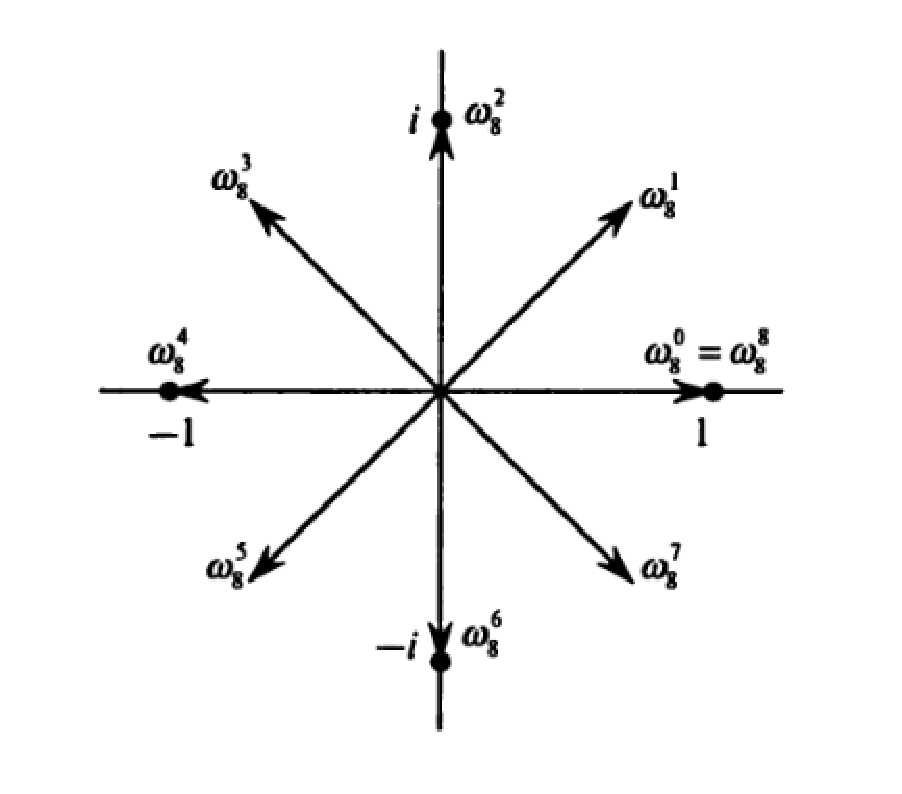
\includegraphics[scale=0.5]{omegas.eps}
    \end{column}
    \begin{column}{.4\textwidth}
      \[
      \begin{split}
        e^{iu}&=\cos(u)+i\sin(u) \\
      \omega_8 &= e^{2\pi i/8}
      \end{split}
      \]
    \end{column}
  \end{columns}
\end{frame}

\frame{
  \frametitle{Лемма о сокращении}
  \begin{rtheorem}
    Для любых целых чисел $n\geq 0$, $k\geq 0$ и $d>0$
\[
\omega^{dk}_{dn}=\omega^k_n
\]
  \end{rtheorem}
\begin{proof}
  \[
  \omega^{dk}_{dn}=\left(e^{2 \pi i/dn}\right)^{dk}=\left(e^{2\pi i/n}\right)^k=\omega_n^k
  \]
\end{proof}
Для любого чётного целого $n>0$
\[
\omega^{n/2}_n=\omega_2=-1
\]
}

\frame{
  \frametitle{Лемма о делении пополам}
\begin{rtheorem}
  Если $n>0$ чётное, то квадраты комплексных корней $n$-й степени из
  единицы представляют собой $n/2$ корней $n/2$-ой степени из
  единицы. 
\end{rtheorem}
\begin{proof}
\[
\begin{split}
  (\omega^k_n)^2 &= \omega_{n/2}^k \\
  (\omega^{k+n/2}_n)^2 &= \omega_n^{2k+n}=\omega_n^{2k}\omega^n_n=\omega^{2k}_n=\left(\omega_n^k\right)^2
\end{split}
\]
Т.е., квадраты $\omega_n^k$ и $\omega^{k+n/2}_n$ одинаковы. 
\end{proof}
}

\frame{
  \frametitle{Лемма о суммировании}
  \begin{rtheorem}
    Для любого целого $n\geq 1$ и ненулевого целого $k$, не кратного
    $n$,
\[
\sum_{j=0}^{n-1}(\omega_n^k)^j=0
\]
  \end{rtheorem}
\begin{proof}
\[
  \sum_{j=0}^{n-1}\left(\omega_n^k\right)^j =
  \frac{(\omega_n^k)^n-1}{\omega_n^k-1} = 
  \frac{(\omega_n^n)^k-1}{\omega_n^k-1} = 
  \frac{1^k-1}{\omega_n^k-1} = 0
\]
\end{proof}
}

\frame[plain]{
  \frametitle{Дискретное преобразование Фурье}
  Полином
  \[
  A(x)=\sum_{j=0}^{n-1}a_jx^j 
  \]
  задан в коэффициентной форме $a=(a_0,a_1, \ldots, a_{n-1})$.
  Нужно вычислить значения $y_k$ в точках $\omega_n^0, \omega_n^1, \ldots,
  \omega_n^{n-1}$:
  \[
  y_k = A(\omega_n^k)=\sum_{j=0}^{n-1}a_j\omega_n^{kj}
  \]
  Вектор $y = (y_0,y_1, \ldots, y_{n-1})$ представляет собой
  дискретное преобразование Фурье вектора $a$:
  \[
  y = \mathrm{DFT}_n(a)
  \]
  Далее будем предполагать, что $n=2^k$ для некоторого $k$. Если это
  не так, то несложно добавить нулевых старших коэффициентов. 
}


\subsection{Быстрое преобразование Фурье}
\frame{
\frametitle{Идея БПФ}
Воспользуемся доказанными свойствами мнимых корней из единицы:
\[
\begin{split}
  A^{[0]}(x) &= a_0 + a_2x + a_4x^2 + \cdots + a_{n-2}x^{n/2-1},\\
  A^{[1]}(x) &= a_1 + a_3x + a_5x^2 + \cdots + a_{n-1}x^{n/2-1}
\end{split}
\]
Тогда задачу вычисления $A(x)$ в точках $\omega_n^0,
\omega_n^1,\ldots,\omega_n^{n-1}$ можно свести к:
\begin{enumerate}
  \item Вычислить $A^{[0]}(x)$ и $A^{[1]}(x)$ степени не выше $n/2$ в
    точках $(\omega_n^0)^2, (\omega_n^1)^2, \ldots,
    (\omega_n^{n-1})^2$
  \item Объединить результаты
\[
A(x)=A^{[0]}(x^2)+xA^{[1]}(x^2)
\]
\end{enumerate}
\pause
Тем самым задача вычисления $\mathrm{DFT}_n$ сведена к вычислению двух задач
$\mathrm{DFT}_{n/2}$.
}

\frame[plain]{
  \frametitle{Рекурсивный БПФ}
  \begin{codebox}
    \Procname{$\proc{Recursive-FFT}(a)$}
    \li $n \gets \id{length}[a]$
    \li \If $n \isequal 1$ 
    \li \Then \Return $a$ \End
    \li $\omega_n \gets e^{2\pi i / n}$
    \li $\omega \gets 1$
    \li $a^{[0]} \gets (a_0, a_2, \ldots, a_{n-2})$
    \li $a^{[1]} \gets (a_1, a_3, \ldots, a_{n-1})$
    \li $y^{[0]} \gets \proc{Recursive-FFT}(a^{[0]})$
    \li $y^{[1]} \gets \proc{Recursive-FFT}(a^{[1]})$
    \li \For $k \gets 0$ \To $n/2-1$ \Do
    \li $y_k \gets y_k^{[0]} + \omega y_k^{[1]}$
    \li $y_{k+(n/2)} \gets y_k^{[0]} - \omega y_k^{[1]}$
    \li $\omega \gets \omega \omega_n$ \End
    \li \Return y
  \end{codebox}
}

\frame{
  \frametitle{Обоснование}
  \begin{enumerate}
    \item Для значений $y_0, y_1, \ldots, y_{n/2-1}$:
\[
\begin{split}
y_k &= y_k^{[0]} + \omega_n^ky_k^{[1]} = A^{[0]}(\omega_{n/2}^{k}) +
\omega_n^kA^{[1]}(\omega_{n/2}^{k}) =\\
&=  A^{[0]}(\omega_n^{2k}) + \omega_n^kA^{[1]}(\omega_n^{2k}) = A(\omega_n^k).
\end{split}
\]
\item Для $y_{n/2}, y_{n/2+1}, \ldots, y_{n-1}$ и $k=0, 1, \ldots,
  n/2-1$:
  \[
  \begin{split}
    y_{k+(n/2)} &= y_k^{[0]} - \omega_n^ky_k^{[1]} = y_k^{[0]} +
    \omega_n^{k+(n/2)}y_k^{[1]} = \\
    &= A^{[0]}(\omega_n^{2k}) +
    \omega_n^{k+(n/2)}A^{[1]}(\omega_n^{2k}) = \\
    &= A^{[0]}(\omega_n^{2k+n}) +
    \omega_n^{k+(n/2)}A^{[1]}(\omega_n^{2k+n}) = \\
    & = A(\omega_n^{k+(n/2)}).
  \end{split}
  \]
  \end{enumerate}
}

\frame{
  \frametitle{Время работы $\proc{Recursive-FFT}$}
  \begin{enumerate}
    \item Собственное время работы $\Theta(n)$, где $n$ --- длина
      исходного вектора.
    \item Реккурентное соотношение времени работы:
\[
T(n)=2T(n/2) + \Theta(n) = \Theta(n\lg n)
\]
  \end{enumerate}
}

\frame{
  \frametitle{Интерполяция во мнимых корнях из единицы}
  ДПФ можно представить как $y=V_na$ где $V_n$ --- матрица Вандермонда
  по степеням $\omega_n$:
\[
\left(
\begin{array}{c}
y_0 \\
y_1 \\
y_2 \\
y_3 \\
\vdots \\
y_{n-1}
\end{array}
\right) = 
    \left( 
\begin{array}{ccccc}
1 & 1 & 1 & \ldots & 1 \\
1 & \omega_n & \omega_n^2 & \ldots & \omega_n^{n-1} \\
1 & \omega_n^2 & \omega_n^4 & \ldots & \omega_n^{2(n-1)} \\
1 & \omega_n^3 & \omega_n^6 & \ldots & \omega_n^{3(n-1)} \\
\vdots & \vdots & \vdots & \ddots & \vdots \\
1 & \omega_{n}^{n-1} & \omega_n^{2(n-1)} & \ldots & \omega_n^{(n-1)(n-1)}
\end{array}
\right)
\left(
\begin{array}{c}
a_0 \\
a_1 \\
a_2 \\
a_3 \\
\vdots \\
a_{n-1}
\end{array}
\right)
\]
\pause

Тогда для выполнения обратной операции $a=\mathrm{DFT}^{-1}(y)$ нужно вычислить
$V_n^{-1}$:
$a = V_n^{-1}y$
}

\frame{
  \begin{rtheorem}
    Для $j,k=0,1,\ldots, n-1$ $(j,k)$-й элемент матрицы $V_n^{-1}$
    равен $\omega_n^{-kj}/n$
  \end{rtheorem}

  \begin{proof}
    Покажем, что в этом случае $V_n^{-1}V_n=I_n$, единичной матрице
    размером $n\times n$. Рассмотрим $(j,j')$-й элемент матрицы
    $V_n^{-1}V_n$:
    \[
    [V_n^{-1}V_n]_{jj'} =
    \sum_{k=0}^{n-1}(\omega_n^{-kj}/n)(\omega_n^{kj'}) = \sum_{k=0}^{n-1}\omega_n^{k(j'-j)}/n
    \]
    По лемме о суммировании эта сумма равна 1, если $j'=j$ и 0 в
    противном случае.  Т.к.  
    \[
    -(n-1)\leq j' -j \leq n-1
    \]
    то $j'-j$ не кратно $n$, т.е. лемма применима. 
  \end{proof}
}

\frame{
  \frametitle{Обратное ДПФ}
  Если дана обратная матрица $V_n^{-1}$, то $\mathrm{DFT}_n^{-1}(y)$
  вычисляется по формуле:
  \[
  a_j=\frac{1}{n}\sum_{k=0}^{n-1}y_k\omega_n^{-kj}, \qquad
  j=0,1,\ldots, n-1
  \]
  \pause
  Алгоритм вычисления аналогичен $\proc{Recursive-FFT}$ с небольшими
  изменениями:
  \begin{enumerate}
  \item Поменять ролями $a$ и $y$.
  \item Заменить $\omega_n$ на $\omega_n^{-1}$.
  \item Разделить каждый элемент результата на $n$.
  \end{enumerate}
}
\frame{
  \frametitle{Теорема о свёртке}
  Тем самым, с помощью прямого и обратного БПФ можно преобразовать
  полином степени не выше $n$ из коэффициентой формы в форму значений
  в точках и обратно за время $\Theta(n\lg n)$. А так же: 
  \begin{rtheorem}
    Для любых двух векторов $a$ и $b$ длины $n$, где $n$ является
    степенью 2, справедливо соотношение:
    \[
    a \otimes b = \mathrm{DFT}_{2n}^{-1}(\mathrm{DFT}_{2n}(a)\cdot \mathrm{DFT}_{2n}(b))
    \]
    где векторы $a$ и $b$ дополняются нулями до длины $2n$, а
    <<$\cdot$>> обозначает покомпонентное произведение двух
    $2n$-элементных векторов. 
  \end{rtheorem}
}

\end{document}
    
